\chapter{Introduction}
\label{sec:intro}
%\chaptermark{Optional running chapter heading}

% The key point here is that data is large and often irregular and we want
% to run complex computation on them.
In today's big data era, we face the challenges in both the explosion of
data volume and the increasing complexity of data analysis. Experiments,
simulations and observations generate terabytes or
even petabytes in many scientific and business areas. After collecting
a massive amount of data, we often need to perform complex data analysis
and machine learning techniques to gain insight from the data. Furthermore,
the fields of data analysis and machine learning evolve rapidly and the community
is developing many new algorithms to effectively extract value from massive
datasets.

% Graph analysis.
A class of commonly used data analysis in both academia and industry is graph
analysis. This models
real-world problems in the form of graphs (vertices and edges) to study objects
and the connection between the objects. Graph analysis becomes ubiquitous
and has applications to many fields such as social networks, semantic search
and knowledge discovery and cybersecurity. A well-known example is that Google
applies PageRank \cite{pagerank} on the Web page graph to determine the importance
of Web pages so that Google can provide users more relevant search results.

When applying graph analysis to real-world problems, we often encounter
massive and irregular graphs. For example, the Facebook social network graph
has billions of vertices, hundreds of billions of edges; the neural network
of a human brain has a fundamental size of $10^{11}$ vertices and $10^{15}$ edges;
graphs that evolve over time can grow even larger. These graphs often have
nearly random vertex connection and power law distribution, which cause random
memory access and load imbalance. As such, leading systems process graph analysis
in RAM and scale to large graphs in a cluster of machines. While good partitions
may be important for performance~\cite{surfer}, these leading systems partition
graphs randomly \cite{powergraph}. Network performance emerges as the bottleneck
and large-scale graph analysis requires fast networks to realize good performance.

% Matrix formulation for graph analysis
Although the lead graph processing frameworks view a graph as a collection of
vertices and edges, we can also represent a graph with a sparse matrix and
express graph analysis
as matrix operations \cite{Mattson13}. In this formulation, a row
or a column of a sparse matrix represents a vertex in a graph and a non-zero
entry encodes the existence of an edge or the edge weight on a graph.
As such, these matrices inherit structure from natural graphs. Specifically,
these matrices are typically very sparse and have near-random distribution
for non-zero entries. They also have a power law distribution that governs
the number of non-zero entries per row and column.

This matrix formulation has several advantages for some graph analysis problems.
First, this formulation is more intuitive for domain experts because users can
express their graph algorithms with high-level matrix operations. The matrix
formulation may also lead to more efficient implementations for some graph
analysis applications such as PageRank \cite{pagerank} and spectral clustering
\cite{spectral}, expressed intuitively with sparse matrix multiplication.
By highly optimizing this matrix operation, we significantly improve
performance of the implementations of many graph algorithms.

% Matrix formulation for general data analysis
Other than graph analysis, linear algebra is another fundamental tool for many
scientific and machine learning applications. In these applications, we store
data in (sparse or dense) matrices, and express algorithms with matrix
operations. Matrix formulation is simple and intuitive for domain experts.
This leads to the development of many popular matrix-oriented programming
frameworks, such as MatLab and R, to help scientists encode and deploy complex
algorithms.

Complex data analysis at a large scale faces significant challenges for
conventional tools. For instance, MatLab and R are known to scale to large
datasets poorly. Even though SQL database systems can process relatively large
datasets, their programming interface is not designed for programming machine
learning algorithms and their internal optimizations are not designed for this
type of workloads either.
The challenges lead to the redesign of data analysis tools.
MapReduce \cite{mapreduce} is one of the most well-known tools developed for
data analysis in the petabyte scale. Even though MapReduce is able to
process data of petabytes in a large cluster, the framework is not able to
handle many data analysis tasks efficiently due to the limited primitive
operations provided by the framework. Since then, many distributed frameworks,
such as Dryad \cite{dryad}, Spark \cite{spark} and Naiad \cite{naiad}, have
been developed for processing large datasets and these frameworks provides
more primitives to express data analysis algorithms more efficiently.
% related work in supercomputing.

Majority of the current research focuses on scaling out to a large cluster,
but many of them achieve better scalability at the cost of large overhead
introduced to the system. This is a common problem in many distributed systems
such as MapReduce. As McSherry et al. \cite{mcsherry15}
points out, many graph analysis frameworks such as PowerGraph \cite{powergraph}
and GraphX \cite{graphx} suffer from the same problem. As such, these systems
are less economical in terms of dollar efficiency and energy efficiency, which
are obstacles of moving to exascale computation.

% I/O
This thesis explores a different direction of scaling data analysis. Instead
of scaling out to a large cluster, we focus on large-scale data analysis in
a single machine, by utilizing the fast I/O technology, and explore
efficient implementations of data analysis tasks for a large parallel machine.

This work is motivated
by the tremendous improvement in storage I/O technology in the recent years.
For example, the latest development of flash memory \cite{fusionio, safs} has
reached over one million random IOPS and over ten gigabytes per second. This
is only one order of magnitude slower than RAM. We believe the advance of
I/O technologies opens a new direction for large-scale data analysis.
The tremendous performance
improvement in I/O potentially makes flash memory the true extension of RAM
and motivates us to develop new frameworks that fully utilize the I/O capacity
for large-scale data analysis.

% The goals of the dissertation.
Given the tremendous hardware improvement, this thesis addresses mainly two
questions: \textit{(i)} Can we replace RAM with fast flash memory in large-scale
data analysis? \textit{(ii)} To what extent
can the performance of flash-based data analysis approach that of RAM-based
data analysis? If data analysis on flash memory can achieve performance comparable to
that in RAM, it will positively affect computer architecture and revolutionize
large-scale data analysis.

In this thesis, we build
efficient programming frameworks with commodity hardware for various
data analysis applications such as graph analysis and machine learning.
%\dz{I need to emphasize the programming framework part.}
This work is orthogonal to the distributed solutions because our work serve as
a building block
for the distributed solutions to process data at even a larger scale.
% point out that our solution in some applications can outperform a pure
% distributed solution.

Hardware advances impose many new challenges in system design (both the operating
system and the data analysis framework). Operating systems were traditionally
designed with an assumption of slow I/O. There exists significant overhead in
almost all layers of the block stack of the Linux kernal when it operates on
fast storage. High-speed random I/O consumes significant CPU power, which
requires us to minimize CPU overhead for I/O access in order to maximize
the overall performance. Although the latest I/O devices deliver unprecedented
performance, they are still much slower than RAM, let alone CPU cache, in both
throughput and latency. As such, it is crucial for data analysis frameworks to
reduce I/O whenever
possible to achieve performance better than the raw hardware delivers.

% currsize is not set in the long table environment, so we need to set it before we set it up.
\makeatletter
\let\@currsize\normalsize
\makeatother

\begin{figure}[t]
\centering
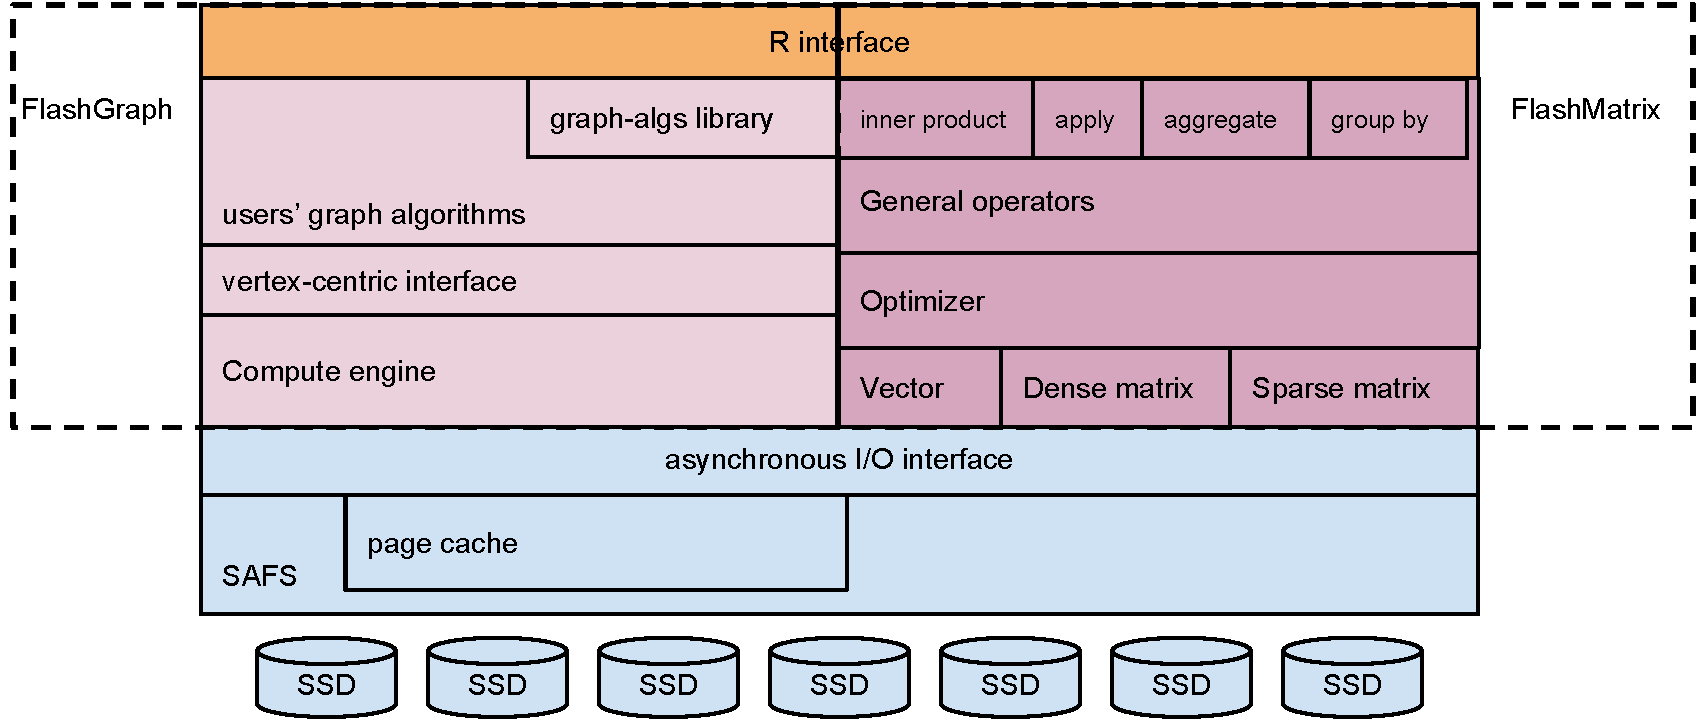
\includegraphics[scale=0.5]{figs/arch.pdf}
\label{fig:arch}
\caption{The architecture of FlashX.}
\end{figure}

We build an SSD-based data analysis ecosystem called FlashX to explore the benefits
that flash memory brings to large-scale data analysis. In this thesis,
we specifically targets graph analysis and machine learning due to their ubiquity.
FlashX has three main subsystems:
\begin{itemize}
	\item SAFS \cite{safs} is a user-space filesystem optimized for large SSD
		arrays. SAFS abstracts away the complexity of data access on SSDs and
		delivers the maximal I/O performance of a large SSD array in a NUMA
		machine. SAFS also provides an efficient caching layer \cite{SA-cache}.
	\item FlashGraph \cite{flashgraph} is a semi-external memory graph analysis
		framework. FlashGraph takes advantage of SAFS and issues I/O requests
		carefully to bring data from SSDs to CPUs efficiently for graph analysis
		to achieve performance comparable to in-memory counterparts. FlashGraph
		is specifically optimized for graph applications that generates random
		I/O access to SSDs.
	\item FlashMatrix implements a set of basic matrix operations as well as
		some generalized matrix operations to express a large range of machine
		learning and data analysis applications in external memory. It supports
		both sparse matrices \cite{SEM_SpMM} and dense matrices \cite{flashmatrix}.
		Like FlashGraph, the goal of FlashMatrix is to brings data from SSDs to
		CPUs efficiently for basic and generalized matrix operations. Unlike
		FlashGraph, FlashMatrix is optimized for applications with sequential
		I/O access to SSDs. FlashMatrix reimplements many matrix operations
		in the R framework to execute R code in parallel and out of core
		automatically.
\end{itemize}

FlashX uses semi-external memory for graph analysis
and matrix computation to achieve both scalability and computation efficiency.
For graph analysis, semi-external memory \cite{Abello98} maintains algorithmic
vertex state in RAM and edge lists on storage. Only using memory for vertices
increases the scalability of graph engines in proportion to the ratio of edges
to vertices in a graph. In FlashMatrix, we introduce a similar construct for
sparse matrix dense matrix multiplication in which one or more columns of
a dense matrix are kept in memory and the sparse matrix is accessed from
external memory. We can even extend this construct to some machine learning
algorithms such as k-means \cite{kmeans}, where some of the intermediate
computation state is kept in memory while input data matrices are stored on
SSDs. For many data analysis tasks, semi-external memory effectively utilizes
memory in a machine to reduce I/O access and achieve performance. In addition,
this computation paradigm reduces the amount of data written to SSDs
dramatically, which is essential to increase the lifetime of SSDs.

This thesis demonstrates that FlashX in semi-external memory realizes
in-memory performance for many data analysis tasks while scaling to massive
datasets in a single machine. FlashGraph in semi-external memory achieves
efficiency comparable to its in-memory version and Galois \cite{galois},
a high-performance, in-memory graph engine with a low-level API, on
a wide-variety of algorithms that generate diverse access patterns, while
significantly outperforming PowerGraph, a popular distributed in-memory
graph engine. We further demonstrate that FlashGraph can process massive
natural graphs in a single machine with relatively small memory footprint;
e.g., we perform breadth-first search on a graph of 3.4 billion vertices
and 129 billion edges using only 22 GB of memory. Similarly, the out-of-core
execution of FlashMatrix achieves performance comparable to the in-memory
execution. The implementations of machine learning algorithms in FlashMatrix
significantly outperforms the same algorithms in Spark MLlib \cite{mllib}.
FlashMatrix effortlessly scales to datasets with billions of data points and
its out-of-core execution uses a small fraction of resources required by
in-memory implementations. Given the fast performance and small memory footprint,
we conclude that FlashX offers unprecedented opportunities for users to perform
massive data analysis efficiently with commodity hardware.

\section{Related work}
% General-purpose data processing framework
MapReduce \cite{mapreduce} led the trend of large-scale data analysis. It
provides a very simple programming interface. Developers only need to provde
a \textit{map} function and
a \textit{reduce} function. The system scales users' computation to very large
datasets in a large cluster and handle machine failures automatically.
The simplicity of its programming interface and the unprecedented scalability
attracted tremendous academic and industrial attention, which leads to
the development of Hadoop \cite{hadoop}, the open-source clone of MapReduce.
MapReduce works very well for simple data processing tasks that can be
partitioned easily and do not require much communication between partitions.
Many data processing tasks at Google, such as count of URL access frequency
and reverse Web links, are tasks that fit the MapReduce programming paradigm.
However, if a task requires significant data exchange between partitions,
MapReduce requires sorting to move data to the right location, which leads
to significant overhead. As such, typical graph algorithms such as breadth-first
search and triangle counting are very slow in MapReduce.

Dryad \cite{dryad} and Naiad \cite{naiad} are distributed execution engine to
process
large datasets. Unlike MapReduce, Dryad provides a much more flexible computation
model and gives developers more fine-grain control over computation and data
communication. Developers construct a directed acyclic graph to describe
communication in the computation and define computation on the vertices in
the graph to express algorithms. Naiad provides an even more
flexible computation model, \textit{timely dataflow}, that supports data flow
graphs with loops. As such, it supports high throughput for batch processing,
low latency for stream processing as well as iterative and incremental
computations. Given the flexible computation model, both Dryad and Naiad
implement varieties of data processing tasks more efficiently at the cost of
higher programming complexity.

Unlike previous distributed frameworks, Spark \cite{spark} is specifically
optimized for in-memory data processing in a distributed environment.
Unlike MapReduce, which relies on writing data to the underlying distributed
filesystem to pass data reliably between MapReduce jobs, Spark keeps data
passed between different computation stages in memory
to avoid overhead of I/O access. Instead of replicating data to achieve
reliability, Spark stores transformation operations associated with RDDs to
reconstruct a lost partition of an RDD due to node failure.

% Programming interface on top of data processing frameworks
Due to the programming complexity in the distributed execution engines, many
programming frameworks have been developed on top of the distributed execution
engines. Pig Latin \cite{pig} and FlumeJava \cite{flumejava} build on top of
MapReduce to provide high-level SQL-like operations for general data analysis.
DryadLINQ \cite{dryadlinq} builds on top of Dryad and exposes a high-level
language to express data analysis tasks. Fundamentally, when these systems
translate high-level operations to low-level primitives, they combine high-level
operations to reduce the number of invocations of low-level primitives as much
as possible. The achievable performance of these programming frameworks is
bound by the underlying distributed execution engines.

% MapReduce-based systems for graph analysis and machine learning.
Given the popularity of MapReduce, many MapReduce-based systems have been
developed to perform graph analysis and machine learning tasks. PEGASUS
\cite{pegasus} is a popular graph processing engine built on MapReduce.
PEGASUS respects the nature of the MapReduce programming paradigm and
expresses
graph algorithms as a generalized form of sparse matrix-vector multiplication.
This form of computation works relatively well for graph algorithms such as
PageRank \cite{pagerank} and label propagation \cite{label_prop}, but performs
poorly for graph traversal algorithms. HEIGEN \cite{heigen} implements
an eigensolver on top of MapReduce for spectral analysis on billion-node
graphs. Despite optimizations in the framework, the HEIGEN eigensolver is
orders of magnitude slower than state-of-art distributed memory eigensolvers.
Cheng-Tao Chu et. al \cite{Chu07} implements a set of machine learning
algorithms using MapReduce to achieve speedup in a multicore machine. SystemML
\cite{systemml} builds a scalable declarative machine learning system on top
of MapReduce, which exposes a declarative higher-level language for writing
ML algorithms.

% Distributed graph processing frameworks
Due to the importance of graph analysis, both industry and academia build
dedicated graph processing frameworks for large-scale graph analysis.
Graph analysis results in a large number of random memory accesses, and
thus state-of-art graph engines use distributed memory for large-scale
graph analysis.
Pregel \cite{pregel} is a distributed graph-processing framework that
allows users to express graph algorithms in vertex-centric programs  
using bulk-synchronous processing (BSP).
It abstracts away the complexity of programming in a distributed-memory 
environment and runs users' code in parallel on a cluster.
Giraph \cite{giraph} is an open-source implementation of Pregel.
GraphLab \cite{graphlab} and PowerGraph \cite{powergraph} prefer shared-memory
to message passing and provide asynchronous execution.
Trinity \cite{trinity} optimizes message passing by restricting vertex
communication to a vertex and its direct neighbors.

% External-memory graph processing frameworks
Despite random memory access required by graph analysis, significant efforts
have been made to scale graph analysis using disks. GraphChi \cite{graphchi}
and X-stream \cite{xstream} are specifically designed for magnetic disks. They
eliminate random data access from disks by scanning the entire graph dataset
in each iteration. Like graph processing frameworks built on top of MapReduce,
they work relatively well for graph algorithms that require computation on all
vertices, but share the same limitations, i.e., suboptimal graph traversal
algorithm performance. TurboGraph \cite{turbograph} is an external-memory graph
engine optimized for SSDs. TurboGraph targets graph algorithms
expressed in sparse matrix vector multiplication, so it is difficult to
implement graph applications such as triangle counting.

% linear algebra for graph analysis
Many graph algorithms can be formulated as sparse matrix multiplication or
generalized sparse matrix multiplication \cite{Mattson13, linear_algebra}.
In this abstraction, PageRank and label propagation are efficiently expressed
as sparse-matrix, dense-vector multiplication, and breadth-first search as 
sparse-matrix, sparse-vector multiplication. KDT \cite{kdt} is a system that
realizes the abstraction and performs graph analysis using linear algebra with
sparse adjacency matrices and vertex-state vectors as data representations.
These frameworks target mathematicians and those with the ability to formulate
and express their problems in the form of linear algebra.

% Additional frameworks for large-scale machine learning.
Many machine learning frameworks have been developed to enable large-scale
machine learning. H2O \cite{h2o} and Spark MLlib \cite{mllib} are machine
learning libraries with a collection of machine learning algorithms implemented
on Spark. GraphLab \cite{graphlab} is a programming framework that provides
primitives for graph-based machine learning algorithms in a distributed
environment. OptiML \cite{optiml} is a domain-specific language and supports
vector, matrix and graph operations to implement machine learning algorithms.
It is built on top of a parallel runtime system called Delite \cite{delite}
to enable parallelism in a heterogeneous computation environment in a single
machine. Petuum \cite{petuum} is a distributed programming framework for
implementing machine learning algorithms. It leverages several fundamental
properties of machine learning algorithms: error tolerance, dynamic structure
and non-uniform convergence, and aims at faster convergence of
an algorithm instead of achieving higher throughput in a single iteration.
